% Options for packages loaded elsewhere
% Options for packages loaded elsewhere
\PassOptionsToPackage{unicode}{hyperref}
\PassOptionsToPackage{hyphens}{url}
\PassOptionsToPackage{dvipsnames,svgnames,x11names}{xcolor}
%
\documentclass[
  letterpaper,
  DIV=11,
  numbers=noendperiod]{scrreprt}
\usepackage{xcolor}
\usepackage{amsmath,amssymb}
\setcounter{secnumdepth}{5}
\usepackage{iftex}
\ifPDFTeX
  \usepackage[T1]{fontenc}
  \usepackage[utf8]{inputenc}
  \usepackage{textcomp} % provide euro and other symbols
\else % if luatex or xetex
  \usepackage{unicode-math} % this also loads fontspec
  \defaultfontfeatures{Scale=MatchLowercase}
  \defaultfontfeatures[\rmfamily]{Ligatures=TeX,Scale=1}
\fi
\usepackage{lmodern}
\ifPDFTeX\else
  % xetex/luatex font selection
\fi
% Use upquote if available, for straight quotes in verbatim environments
\IfFileExists{upquote.sty}{\usepackage{upquote}}{}
\IfFileExists{microtype.sty}{% use microtype if available
  \usepackage[]{microtype}
  \UseMicrotypeSet[protrusion]{basicmath} % disable protrusion for tt fonts
}{}
\makeatletter
\@ifundefined{KOMAClassName}{% if non-KOMA class
  \IfFileExists{parskip.sty}{%
    \usepackage{parskip}
  }{% else
    \setlength{\parindent}{0pt}
    \setlength{\parskip}{6pt plus 2pt minus 1pt}}
}{% if KOMA class
  \KOMAoptions{parskip=half}}
\makeatother
% Make \paragraph and \subparagraph free-standing
\makeatletter
\ifx\paragraph\undefined\else
  \let\oldparagraph\paragraph
  \renewcommand{\paragraph}{
    \@ifstar
      \xxxParagraphStar
      \xxxParagraphNoStar
  }
  \newcommand{\xxxParagraphStar}[1]{\oldparagraph*{#1}\mbox{}}
  \newcommand{\xxxParagraphNoStar}[1]{\oldparagraph{#1}\mbox{}}
\fi
\ifx\subparagraph\undefined\else
  \let\oldsubparagraph\subparagraph
  \renewcommand{\subparagraph}{
    \@ifstar
      \xxxSubParagraphStar
      \xxxSubParagraphNoStar
  }
  \newcommand{\xxxSubParagraphStar}[1]{\oldsubparagraph*{#1}\mbox{}}
  \newcommand{\xxxSubParagraphNoStar}[1]{\oldsubparagraph{#1}\mbox{}}
\fi
\makeatother


\usepackage{longtable,booktabs,array}
\usepackage{calc} % for calculating minipage widths
% Correct order of tables after \paragraph or \subparagraph
\usepackage{etoolbox}
\makeatletter
\patchcmd\longtable{\par}{\if@noskipsec\mbox{}\fi\par}{}{}
\makeatother
% Allow footnotes in longtable head/foot
\IfFileExists{footnotehyper.sty}{\usepackage{footnotehyper}}{\usepackage{footnote}}
\makesavenoteenv{longtable}
\usepackage{graphicx}
\makeatletter
\newsavebox\pandoc@box
\newcommand*\pandocbounded[1]{% scales image to fit in text height/width
  \sbox\pandoc@box{#1}%
  \Gscale@div\@tempa{\textheight}{\dimexpr\ht\pandoc@box+\dp\pandoc@box\relax}%
  \Gscale@div\@tempb{\linewidth}{\wd\pandoc@box}%
  \ifdim\@tempb\p@<\@tempa\p@\let\@tempa\@tempb\fi% select the smaller of both
  \ifdim\@tempa\p@<\p@\scalebox{\@tempa}{\usebox\pandoc@box}%
  \else\usebox{\pandoc@box}%
  \fi%
}
% Set default figure placement to htbp
\def\fps@figure{htbp}
\makeatother





\setlength{\emergencystretch}{3em} % prevent overfull lines

\providecommand{\tightlist}{%
  \setlength{\itemsep}{0pt}\setlength{\parskip}{0pt}}



 


\KOMAoption{captions}{tableheading}
\makeatletter
\@ifpackageloaded{bookmark}{}{\usepackage{bookmark}}
\makeatother
\makeatletter
\@ifpackageloaded{caption}{}{\usepackage{caption}}
\AtBeginDocument{%
\ifdefined\contentsname
  \renewcommand*\contentsname{Table of contents}
\else
  \newcommand\contentsname{Table of contents}
\fi
\ifdefined\listfigurename
  \renewcommand*\listfigurename{List of Figures}
\else
  \newcommand\listfigurename{List of Figures}
\fi
\ifdefined\listtablename
  \renewcommand*\listtablename{List of Tables}
\else
  \newcommand\listtablename{List of Tables}
\fi
\ifdefined\figurename
  \renewcommand*\figurename{Figure}
\else
  \newcommand\figurename{Figure}
\fi
\ifdefined\tablename
  \renewcommand*\tablename{Table}
\else
  \newcommand\tablename{Table}
\fi
}
\@ifpackageloaded{float}{}{\usepackage{float}}
\floatstyle{ruled}
\@ifundefined{c@chapter}{\newfloat{codelisting}{h}{lop}}{\newfloat{codelisting}{h}{lop}[chapter]}
\floatname{codelisting}{Listing}
\newcommand*\listoflistings{\listof{codelisting}{List of Listings}}
\makeatother
\makeatletter
\makeatother
\makeatletter
\@ifpackageloaded{caption}{}{\usepackage{caption}}
\@ifpackageloaded{subcaption}{}{\usepackage{subcaption}}
\makeatother
\usepackage{bookmark}
\IfFileExists{xurl.sty}{\usepackage{xurl}}{} % add URL line breaks if available
\urlstyle{same}
\hypersetup{
  pdftitle={Muhammad Farrel Wibowo},
  pdfauthor={13523153 Muhammad Farrel Wibowo},
  colorlinks=true,
  linkcolor={blue},
  filecolor={Maroon},
  citecolor={Blue},
  urlcolor={Blue},
  pdfcreator={LaTeX via pandoc}}


\title{Muhammad Farrel Wibowo}
\usepackage{etoolbox}
\makeatletter
\providecommand{\subtitle}[1]{% add subtitle to \maketitle
  \apptocmd{\@title}{\par {\large #1 \par}}{}{}
}
\makeatother
\subtitle{Portfolio Asesmen II-2100 KIPP}
\author{13523153 Muhammad Farrel Wibowo}
\date{2027-07-10}
\begin{document}
\maketitle

\renewcommand*\contentsname{Table of contents}
{
\hypersetup{linkcolor=}
\setcounter{tocdepth}{2}
\tableofcontents
}

\bookmarksetup{startatroot}

\chapter*{Selamat Berjumpa}\label{selamat-berjumpa}
\addcontentsline{toc}{chapter}{Selamat Berjumpa}

\markboth{Selamat Berjumpa}{Selamat Berjumpa}

\begin{figure}[H]

{\centering \includegraphics[width=9.5\linewidth,height=\textheight,keepaspectratio]{../images/profile-pict.png}

}

\caption{About Me}

\end{figure}%

Muhammad Farrel Wibowo adalah mahasiswa Teknik Informatika Institut
Teknologi Bandung angkatan 2023. Lahir di Jakarta pada 18 Juni 2005,
kini menetap di Jatinangor untuk menjalani aktivitas perkuliahan,
sementara rumah keluarganya masih berada di Jakarta. Sejak kecil Farrel
sudah akrab dengan dunia teknologi---mulai dari smartphone, komputer,
hingga internet---yang menumbuhkan rasa ingin tahu tentang bagaimana
teknologi bekerja dan bagaimana ia dapat mengubah kehidupan manusia.

Sehari-hari, Farrel dikenal sebagai sosok yang disiplin, pekerja keras,
dan reflektif. Ia memiliki berbagai hobi seperti olahraga gym,
fotografi, otomotif, videografi, dan tenis. Namun di balik banyaknya
minat tersebut, benang merah yang mengikat semuanya adalah rasa ingin
belajar dan berkembang secara berkelanjutan.

\bookmarksetup{startatroot}

\chapter{UTS-1 All About Me}\label{uts-1-all-about-me}

\begin{figure}[H]

{\centering \includegraphics[width=9.5\linewidth,height=\textheight,keepaspectratio]{All_About_me/../images/profile-pict.jpeg}

}

\caption{About Me}

\end{figure}%

Muhammad Farrel Wibowo adalah mahasiswa Teknik Informatika Institut
Teknologi Bandung angkatan 2023. Lahir di Jakarta pada 18 Juni 2005,
kini menetap di Jatinangor untuk menjalani aktivitas perkuliahan,
sementara rumah keluarganya masih berada di Jakarta. Sejak kecil Farrel
sudah akrab dengan dunia teknologi---mulai dari smartphone, komputer,
hingga internet---yang menumbuhkan rasa ingin tahu tentang bagaimana
teknologi bekerja dan bagaimana ia dapat mengubah kehidupan manusia.

Sehari-hari, Farrel dikenal sebagai sosok yang disiplin, pekerja keras,
dan reflektif. Ia memiliki berbagai hobi seperti olahraga gym,
fotografi, otomotif, videografi, dan tenis. Namun di balik banyaknya
minat tersebut, benang merah yang mengikat semuanya adalah rasa ingin
belajar dan berkembang secara berkelanjutan.

\section{\texorpdfstring{\textbf{Kisah yang Membentuk Diri Anda:
Mengenal Kekuatan Identitas
Naratif}}{Kisah yang Membentuk Diri Anda: Mengenal Kekuatan Identitas Naratif}}\label{kisah-yang-membentuk-diri-anda-mengenal-kekuatan-identitas-naratif}

Saya percaya bahwa setiap orang adalah pencerita alami yang menenun
kehidupannya menjadi sebuah kisah. Bagi saya, kisah itu dimulai dari
rasa ingin tahu yang sederhana terhadap teknologi, lalu berkembang
menjadi perjalanan penuh pembelajaran, perjuangan, dan pemaknaan diri.

Di masa SMA di MAN 4 Jakarta, saya mengambil jurusan Sains dan
Matematika dengan kurikulum Cambridge AS Level. Dari situlah saya mulai
memadukan logika dengan kreativitas. Saya bergabung di klub robotika dan
klub teknologi informasi, di mana saya belajar membangun robot serta
memprogramnya dengan Arduino IDE. Salah satu momen berharga adalah
ketika tim saya berhasil meraih medali perak pada ASEAN Innovative
Science \& Entrepreneur Fair (AISEF) berkat proyek Early Warning Flood
System berbasis Arduino, Wi-Fi, dan Blynk. Kemenangan itu bukan sekadar
prestasi, tetapi momen berkilau---saat saya menyadari bahwa teknologi
bukan hanya tentang kode dan alat, melainkan tentang solusi yang
menyentuh kehidupan manusia.

\subsection{\texorpdfstring{\textbf{1. Tiga Lapisan Diri Anda: Di Mana
Cerita Hidup Anda
Berada?}}{1. Tiga Lapisan Diri Anda: Di Mana Cerita Hidup Anda Berada?}}\label{tiga-lapisan-diri-anda-di-mana-cerita-hidup-anda-berada}

Mengikuti kerangka dari Dan P. McAdams, saya bisa memetakan perjalanan
diri saya sebagai berikut:

Level 1: Sifat Dasar. Saya cenderung disiplin, logis, dan berorientasi
pada hasil. Namun, di balik itu saya juga reflektif dan tenang---lebih
banyak mengamati sebelum bertindak.

Level 2: Kepedulian Pribadi. Nilai yang saya pegang adalah tanggung
jawab terhadap proses dan keberanian untuk menghadapi kegagalan. Saya
percaya bahwa setiap kesalahan adalah bentuk pembelajaran yang penting.

Level 3: Identitas Naratif. Inilah titik di mana seluruh lapisan diri
saya bertemu. Saya melihat diri saya sebagai seseorang yang terus
belajar dari masa lalu, memperjuangkan apa yang diinginkan, dan berusaha
berkontribusi lewat teknologi yang bermanfaat bagi orang lain.

Salah satu peristiwa yang paling membentuk identitas saya adalah ketika
saya gagal masuk perguruan tinggi melalui jalur SNBT. Kegagalan itu
sempat menimbulkan rasa kecewa, tetapi justru menjadi titik balik. Saya
belajar untuk bangkit, berjuang kembali melalui jalur Mandiri ITB, dan
akhirnya diterima di jurusan impian saya. Perjalanan itu mengajarkan
bahwa hasil besar tidak datang dari keberuntungan, melainkan dari
konsistensi dan keyakinan.

\subsection{\texorpdfstring{\textbf{2. Pola-Pola Kisah Kehidupan: Apa
yang Membuat Sebuah Cerita
Bermanfaat?}}{2. Pola-Pola Kisah Kehidupan: Apa yang Membuat Sebuah Cerita Bermanfaat?}}\label{pola-pola-kisah-kehidupan-apa-yang-membuat-sebuah-cerita-bermanfaat}

Cerita hidup saya mencerminkan pola penebusan (redemption)---dari
kegagalan menuju keberhasilan, dari keterbatasan menuju kesempatan baru.
Kegagalan masuk kampus favorit bukan akhir cerita, tetapi bab pembuka
dari narasi yang lebih bermakna. Kini, setelah menjadi mahasiswa, saya
juga mulai mengembangkan pola agensi dan koneksi, di mana peran saya
tidak lagi sebatas individu yang berjuang, tetapi bagian dari ekosistem
yang saling tumbuh bersama.

\begin{longtable}[]{@{}
  >{\raggedright\arraybackslash}p{(\linewidth - 2\tabcolsep) * \real{0.2097}}
  >{\raggedright\arraybackslash}p{(\linewidth - 2\tabcolsep) * \real{0.7903}}@{}}
\toprule\noalign{}
\endhead
\bottomrule\noalign{}
\endlastfoot
\textbf{Pola Naratif} & \textbf{Dampak Psikologis dan Pembelajaran
Pribadi} \\
\textbf{Penebusan} (Negatif → Positif) & Gagal di SNBT menjadi titik
balik untuk membangun ketekunan dan rasa percaya diri dalam meraih ITB
melalui jalur mandiri. \\
\textbf{Agensi} (Diri sebagai Aktor Efektif) & Mengembangkan kemampuan
kepemimpinan, pengambilan keputusan, dan inisiatif, seperti saat
memimpin proyek di TEC dan mengikuti hackathon. \\
\textbf{Koneksi} (Hubungan \& Rasa Memiliki) & Menemukan makna dalam
kerja sama tim dan kontribusi kolektif, misalnya saat menjadi staf HMIF
dan anggota ITB Jazz. \\
\textbf{Momen Berkilau} & Juara 3 \textbf{Hackathon} pertama saya di
perkuliahan menjadi simbol bagaimana kolaborasi, kecepatan berpikir, dan
disiplin teknis dapat membawa hasil. \\
\end{longtable}

\subsection{\texorpdfstring{\textbf{3. Seni Memberi Makna: Kekuatan
Super Anda dalam
Bernalar}}{3. Seni Memberi Makna: Kekuatan Super Anda dalam Bernalar}}\label{seni-memberi-makna-kekuatan-super-anda-dalam-bernalar}

Saya tidak pernah menganggap kesalahan sebagai musuh, melainkan guru.
Setiap kegagalan---baik dalam ujian, proyek, maupun
keputusan---membentuk cara berpikir saya yang lebih tenang dan
strategis. Selama berkuliah di ITB, saya menyadari bahwa menjadi
mahasiswa bukan hanya tentang menguasai algoritma atau pemrograman,
tetapi juga belajar bagaimana berpikir jernih di tengah tekanan dan
berinteraksi dengan berbagai karakter.

Momentum baru saya hadir ketika tim kami meraih Juara 3
Hackathon---lomba pertama saya selama kuliah. Selain validasi kerja tim,
kompetisi ini memberikan pembelajaran yang sangat praktis:

Framing masalah \& scoping MVP: menajamkan batas solusi agar berdampak
nyata dalam waktu terbatas.

Kolaborasi teknis di bawah tekanan waktu: branching Git yang rapi, code
review singkat namun tegas, dan keberanian membuat trade-off teknis.

Integrasi cepat \& reliability dasar: mengikat API, merapikan error
handling, serta memastikan demo berjalan stabil.

Storytelling produk: menyusun pitch yang jelas---dari problem statement,
insight pengguna, ke nilai guna---tanpa gimmick berlebihan.

Pengalaman ini menegaskan kembali bahwa agensi bukan semata kemampuan
teknis, melainkan keputusan-keputusan kecil yang konsisten: memilih
prioritas, menjaga ritme tim, dan bertanggung jawab atas kualitas hasil.

Kesadaran terbesar saya tetap sama: dunia ini tidak berputar di sekitar
diri saya sendiri. Setiap orang memiliki kisah, perjuangan, dan maknanya
masing-masing. Menyadari hal ini membuat saya lebih menghargai
keberagaman dan lebih rendah hati dalam proses belajar maupun
berorganisasi. Dari sinilah lahir keseimbangan antara ambisi dan empati.

\subsection{\texorpdfstring{\textbf{4. Mulai Menulis Ulang Kisah Anda:
Dua Langkah
Praktis}}{4. Mulai Menulis Ulang Kisah Anda: Dua Langkah Praktis}}\label{mulai-menulis-ulang-kisah-anda-dua-langkah-praktis}

Meskipun masa lalu tidak bisa diubah, saya menyadari bahwa cara saya
memaknainya bisa. Ada dua langkah yang terus saya latih agar tetap
tumbuh:

\subsubsection{Langkah 1: Eksternalisasi
Masalah}\label{langkah-1-eksternalisasi-masalah}

Saya belajar memisahkan identitas diri dari permasalahan yang saya
hadapi. Alih-alih berpikir ``saya gagal'', saya membingkai ulang menjadi
``saya sedang berhadapan dengan tantangan yang bisa saya atasi.''
Pergeseran cara berpikir ini mengubah rasa frustrasi menjadi ruang untuk
analisis dan perbaikan. Di dunia teknologi yang penuh trial-error,
kemampuan ini membuat saya lebih stabil dan berorientasi solusi.

\subsubsection{Langkah 2: Temukan Momen
Berkilau}\label{langkah-2-temukan-momen-berkilau}

Setiap kali saya merasa kehilangan arah, saya mencari kembali ``momen
berkilau'' yang pernah saya alami:

Ketika saya lolos ITB lewat jalur mandiri setelah gagal SNBT.

Saat dipercaya menjadi mentor di TEC untuk program pembelajaran data
science.

Ketika tim saya memenangkan Juara 3 Hackathon, yang memperkuat keyakinan
bahwa kerja keras kolektif dan visi yang jelas mampu mengubah tekanan
menjadi prestasi.

Momen-momen ini menjadi jangkar optimisme yang saya pegang, sekaligus
bukti bahwa perubahan naratif selalu mungkin.

\subsection{\texorpdfstring{\textbf{5. Kesimpulan: Kisah Saya Masih
Terus
Ditulis}}{5. Kesimpulan: Kisah Saya Masih Terus Ditulis}}\label{kesimpulan-kisah-saya-masih-terus-ditulis}

Perjalanan saya hingga saat ini bukanlah kisah yang sempurna, tetapi
kisah yang jujur. Saya belajar bahwa makna hidup tidak selalu datang
dari hasil yang besar, tetapi dari proses memahami diri sendiri dan
berkontribusi bagi sekitar.

Teknologi mungkin adalah bahasa yang saya pilih untuk mengekspresikan
diri, tetapi nilai yang ingin saya bawa jauh melampaui kode dan
algoritma---yakni ketekunan, rasa syukur, dan kesadaran bahwa setiap
keberhasilan adalah hasil dari perjuangan bersama.

Saya percaya bahwa kisah saya baru saja dimulai. Dan seperti dalam
setiap baris kode yang saya tulis, selalu ada ruang untuk perbaikan,
pembaruan, dan versi yang lebih baik dari diri saya sendiri.

\bookmarksetup{startatroot}

\chapter{UTS-2 My Songs for You}\label{uts-2-my-songs-for-you}

Dari Hati Performed by

Club Eighties

\url{https://youtu.be/USF8xr4QEa0?si=tu8tP-XTlD5Bz-b9}

\subsubsection{Makna dan Alasan Pemilihan
Lagu}\label{makna-dan-alasan-pemilihan-lagu}

Lagu ``Dari Hati'' dipilih karena memiliki makna yang sangat mendalam
tentang kejujuran, kesungguhan, dan ketulusan dalam mencintai seseorang.
Bagi saya, lagu ini menggambarkan bentuk cinta yang sederhana, jujur,
dan tanpa syarat---cinta yang tidak dibungkus oleh ambisi atau
kepemilikan, melainkan oleh keberanian untuk mengungkapkan perasaan yang
paling murni: ``Ku ingin jujur apa adanya, dari hati.''

Lagu ini menjadi inspirasi sekaligus refleksi untuk karya pribadi saya,
``My Songs for U'', yaitu sebuah lagu yang saya tulis dan ingin
nyanyikan pada hari pernikahan saya nanti. Lagu itu bukan sekadar
persembahan musik, tetapi bentuk nyata dari doa dan perasaan terdalam
terhadap pasangan saya kelak---bahwa cinta yang baik tidak perlu banyak
kata, cukup datang dari hati dan dijaga dengan sepenuh hati.

Seperti dalam lirik ``Dari Hati'', kejujuran menjadi fondasi yang saya
yakini harus hadir dalam setiap hubungan. Bagian ``Ku ingin kau menjadi
milikku, entah bagaimana caranya'' tidak dimaknai sebagai kepemilikan
egoistik, melainkan sebagai bentuk niat tulus untuk berbagi perjalanan
hidup bersama seseorang yang kita yakini sebagai belahan hati. Lirik
tersebut juga menandakan kerendahan hati di tengah ketidakpastian, bahwa
cinta tidak selalu bisa dikontrol, namun dapat dijaga dengan keikhlasan.

Bagi saya, lagu ini adalah narasi cinta dewasa---tentang seseorang yang
tidak lagi ingin menaklukkan, melainkan berjuang bersama; yang tidak
lagi bicara tentang ``aku dan kamu'', tetapi tentang ``kita''. Itulah
sebabnya saya ingin mengabadikan semangat yang sama melalui lagu ``My
Songs for U'', yang kelak akan saya nyanyikan pada hari pernikahan saya
sebagai simbol perjalanan hidup yang berpuncak pada makna: mencintai
dengan jujur, dari hati.

{[}Intro{]} Andai engkau tahu Bila menjadi aku, sejuta rasa di hati Lama
tlah kupendam Tapi akan kucoba mengatakannya

{[}Verse 1{]} Ku ingin kau menjadi milikku Entah bagaimana caranya
Lihatlah mataku untuk memintamu Ku ingin jalani bersamamu Coba dengan
sepenuh hati Ku ingin jujur apa adanya Dari hati

{[}Chorus 1{]} Kini engkau tahu aku menginginkanmu Tapi takkan
kupaksakan Dan kupastikan kau belahan hati Bila milikku oooo Ku ingin
kau menjadi milikku Entah bagaimana caranya Lihatlah mataku untuk
memintamu Aku ingin jalani bersamamu Coba dengan sepenuh hati Ku ingin
jujur apa adanya

{[}Bridge{]} Menarilah bersamaku Dengan bintang-bintang Sambutlah diriku
Untuk memelukmu

{[}Chorus 2{]} Ku ingin kau menjadi milikku Entah bagaimana caranya
Lihatlah mataku untuk memintamu Ku ingin jalani bersamamu Coba dengan
sepenuh hati Ku ingin jujur apa adanya Dari hati

{[}Outro{]} Dari hati

\bookmarksetup{startatroot}

\chapter{UTS-3 My Stories for You}\label{uts-3-my-stories-for-you}

\section{\texorpdfstring{\textbf{Sebuah Kisah: ``Belajar Menemukan Diri
di Tengah
Perjalanan''}}{Sebuah Kisah: ``Belajar Menemukan Diri di Tengah Perjalanan''}}\label{sebuah-kisah-belajar-menemukan-diri-di-tengah-perjalanan}

Hidup saya bukan rangkaian kemenangan, melainkan rangkaian proses
memahami arti kegagalan, kesabaran, dan keyakinan. Setiap langkah kecil
membawa pelajaran baru---dan kisah inilah yang ingin saya bagikan, bukan
karena sempurna, tetapi karena ia jujur dan membentuk siapa saya
sekarang.

\begin{center}\rule{0.5\linewidth}{0.5pt}\end{center}

\subsection{\texorpdfstring{\textbf{Awal
Perjalanan}}{Awal Perjalanan}}\label{awal-perjalanan}

Saya tumbuh sebagai anak yang selalu penasaran pada teknologi. Dari
komputer, internet, hingga robotik di SMA, semua itu membuat saya kagum
pada bagaimana sesuatu bisa ``hidup'' karena logika dan kode. Namun di
balik rasa ingin tahu itu, saya sering merasa belum cukup baik. Saya
takut gagal, takut tidak memenuhi ekspektasi.

Kegagalan pertama besar yang saya rasakan adalah saat tidak lolos
\textbf{SNBT}, ujian masuk perguruan tinggi yang selama ini saya
harapkan. Hari itu saya merasa dunia berhenti. Tetapi justru di titik
itu saya belajar makna \emph{penebusan}. Saya belajar bahwa hidup tidak
selalu harus berjalan lurus; kadang kita harus tersesat dulu untuk
benar-benar menemukan arah. Saya memutuskan mencoba jalur
\textbf{Mandiri ITB}, dan berhasil diterima di jurusan impian saya:
\textbf{Teknik Informatika Institut Teknologi Bandung}.

Sejak saat itu, saya memahami bahwa kegagalan bukan akhir cerita---ia
hanyalah tanda bahwa saya sedang ditulis ulang menjadi versi diri yang
lebih baik.

\begin{center}\rule{0.5\linewidth}{0.5pt}\end{center}

\subsection{\texorpdfstring{\textbf{Proses dan
Pembelajaran}}{Proses dan Pembelajaran}}\label{proses-dan-pembelajaran}

Perkuliahan di ITB bukan hanya tentang memahami algoritma atau teori,
tapi tentang membangun daya tahan mental. Di sinilah saya belajar
pentingnya keseimbangan antara ambisi dan empati.\\
Saya belajar menata waktu, menahan ego, menerima perbedaan cara
berpikir, dan memahami bahwa kesuksesan kolektif sering kali lebih
bermakna daripada kemenangan pribadi.

Puncak pengalaman itu datang ketika tim saya meraih \textbf{Juara 3
Hackathon pertama saya di bangku kuliah}.\\
Lomba itu bukan sekadar kompetisi, tapi ujian nyata tentang bagaimana
sebuah ide bisa diwujudkan di bawah tekanan waktu dan perbedaan
pendapat. Saya belajar banyak hal:\\
- Bahwa komunikasi adalah inti dari kolaborasi.\\
- Bahwa keputusan kecil, seperti siapa yang menulis kode terakhir atau
siapa yang mempresentasikan produk, bisa menentukan keberhasilan
bersama.\\
- Bahwa ketenangan dan rasa saling percaya lebih berharga daripada
kecepatan.

Sejak hari itu, saya menyadari bahwa kompetisi sejati bukan antara saya
dan orang lain---melainkan antara saya dan versi diri saya kemarin.

\begin{center}\rule{0.5\linewidth}{0.5pt}\end{center}

\subsection{\texorpdfstring{\textbf{Makna dan Inspirasi untuk Orang
Lain}}{Makna dan Inspirasi untuk Orang Lain}}\label{makna-dan-inspirasi-untuk-orang-lain}

Dari setiap perjalanan itu, saya ingin membagikan satu pesan
sederhana:\\
\textgreater{} ``Hidup tidak akan selalu berjalan sesuai rencana, tetapi
rencana Tuhan selalu berjalan sesuai kebutuhan kita.''

Kegagalan, kehilangan, bahkan ketidakpastian, semuanya adalah ruang
belajar untuk menemukan siapa diri kita sebenarnya.\\
Saya percaya bahwa setiap orang punya cerita yang bisa menyembuhkan
orang lain.\\
Dan jika kisah saya bisa membuat satu orang saja merasa lebih kuat untuk
bangkit, maka perjalanan ini sudah cukup berarti.

\begin{center}\rule{0.5\linewidth}{0.5pt}\end{center}

\subsection{\texorpdfstring{\textbf{Penutup: My Stories for
You}}{Penutup: My Stories for You}}\label{penutup-my-stories-for-you}

Lagu \emph{``Dari Hati''} yang saya pilih di tugas sebelumnya dan kisah
ini memiliki benang merah yang sama---\emph{kejujuran.}\\
Baik dalam cinta maupun dalam hidup, hanya kejujuran yang mampu menuntun
kita pada makna sejati.

Maka ``My Stories for You'' bukan hanya cerita tentang saya,\\
tetapi tentang keberanian untuk tetap percaya,\\
tentang proses menemukan arah di tengah ketidakpastian,\\
dan tentang bagaimana setiap kegagalan dapat berubah menjadi awal dari
sesuatu yang indah---\\
selama dijalani \textbf{dari hati.}

\bookmarksetup{startatroot}

\chapter{UTS-4 My SHAPE (Spiritual Gifts, Heart, Abilities, Personality,
Experiences)}\label{uts-4-my-shape-spiritual-gifts-heart-abilities-personality-experiences}

\begin{quote}
\textbf{Tujuan:} Merangkum rancangan diri (charter) agar saya melayani,
berkarya, dan memimpin secara paling selaras dengan karunia dan
pengalaman hidup saya. Dapat langsung ditempel ke halaman \textbf{UTS-4
--- My SHAPE} dan dipakai sebagai acuan aksi 90 hari.
\end{quote}

\section{\texorpdfstring{Sumber
\href{StrengthsProfile-Muhammad-Farrel.pdf}{VIA
assessment}}{Sumber VIA assessment}}\label{sumber-via-assessment}

\section{0) Ringkasan 1 Halaman}\label{ringkasan-1-halaman}

\textbf{Peran Inti:} Builder--Mentor Technologist --- pembuat solusi
nyata berbasis software/hardware yang tumbuh lewat kolaborasi, lalu
membagikannya ke komunitas (teman seangkatan, adik tingkat, dan
komunitas kampus). \textbf{Misi:} Mengubah rasa ingin tahu menjadi karya
yang bermanfaat---menghadirkan produk kecil yang memecahkan masalah
nyata, sambil membangun diri dan orang lain (belajar bersama, saling
dorong). \textbf{Kekuatan Utama:} disiplin \& ketekunan, kejujuran,
sense of fairness \& tim, kepemimpinan kolaboratif, pertimbangan logis,
harapan \& antusiasme, product thinking cepat. (dikonfirmasi oleh VIA:
Spiritualitas, Keadilan, Pertimbangan, Kepemimpinan, Kerja Tim,
Kejujuran, Kebaikan, Aturan Diri, Kasih, Ketekunan, dll.) \textbf{Dampak
yang Dituju:} mini-produk dan proyek kampus yang ship-able, kolaborasi
sehat, serta kultur belajar yang suportif (di TEC/HMIF/komunitas IF).

\textbf{Peta SHAPE (singkat):}

\begin{itemize}
\tightlist
\item
  \textbf{S --- Spiritual Gifts:} Encouragement/Exhortation, Serving,
  Leadership (kolaboratif), Teaching awal (peer tutoring).
\item
  \textbf{H --- Heart (Minat \& Cinta Pelayanan):} hands-on teknologi
  (AI/aplikasi web/IoT ringan), kompetisi \& hackathon, konten kreatif
  (foto--video), olahraga untuk disiplin diri.
\item
  \textbf{A --- Abilities (Kemampuan):}rapid prototyping (React/Next
  atau Python/Flask/FastAPI), integrasi API, Git workflow, presentasi \&
  demo storytelling, produksi konten (editing).
\item
  \textbf{P --- Personality (Gaya Kepribadian Kerja):} adil \&
  tim-oriented, reflektif-logis, jujur, disiplin, hopeful-energetic;
  nyaman memimpin saat perlu, tetap rendah hati.
\item
  \textbf{E --- Experiences (Pengalaman Kunci):}AISEF Silver (Arduino
  Wi-Fi-Blynk flood warning), klub robotik/ICT/band, Juara 3 Hackathon
  (kuliah), proyek komunitas (TEC/HMIF/ITB Jazz), hobi kreatif \&
  olahraga.
\end{itemize}

\begin{center}\rule{0.5\linewidth}{0.5pt}\end{center}

\section{1) S --- Spiritual Gifts (Karunia
Rohani)}\label{s-spiritual-gifts-karunia-rohani}

\begin{itemize}
\tightlist
\item
  \textbf{Teaching \& Wisdom/Discernment:} cenderung menguatkan tim,
  bantu rekan saat stuck, senang berbagi how-to.
\item
  \textbf{Leadership \& Administration:} menjaga kekompakan, membagi
  peran, fokus ship; cocok jadi squad lead kecil.
\item
  \textbf{Teaching (pemula/peer):} nyaman menjelaskan langkah praktis
  (setup, integrasi API, debug tactics) pada adik tingkat.
\end{itemize}

\begin{center}\rule{0.5\linewidth}{0.5pt}\end{center}

\section{2) H --- Heart (Minat, Nilai,
Kepedulian)}\label{h-heart-minat-nilai-kepedulian}

\begin{itemize}
\item
  \textbf{Teknologi praktis yang ``jadi barang'':} web/app ringan, AI
  kecil yang terasa gunanya, IoT sederhana.
\item
  \textbf{Kompetisi \& hackathon:} senang ritme cepat, scoping MVP, dan
  demo day.
\item
  \textbf{Kreativitas visual:} fotografi--videografi untuk dokumentasi
  tim/produk.
\item
  \textbf{Keseimbangan hidup:} olahraga (gym, tenis) untuk disiplin \&
  fokus.
\item
  \textbf{Nilai utama:} keadilan, kejujuran, dan team first (adil dalam
  pembagian kredit/kerja).
\end{itemize}

\textbf{Masalah yang ingin dipecahkan:}

\begin{center}\rule{0.5\linewidth}{0.5pt}\end{center}

\section{3) A --- Abilities (Kemampuan
Andal)}\label{a-abilities-kemampuan-andal}

\begin{itemize}
\item
  \textbf{Teknis:}
\item
  Rapid prototyping (frontend/backend sederhana), integrasi API, auth
  dasar, error handling seperlunya.
\item
  IoT ringan (warisan AISEF: Arduino + konektivitas), otomasi kecil.
\item
  Git branch--PR--review cepat; pitching \& live demo.
\item
  \textbf{Kreatif \& Komunikasi:} video editing, visual asset untuk
  launch/demo.
\item
  \textbf{Tim \& Eksekusi:} scoping, time-boxing, menjaga ritme stand-up
  singkat, trade-off teknis jelas.
\end{itemize}

\begin{center}\rule{0.5\linewidth}{0.5pt}\end{center}

\section{4) P --- Personality (Gaya Kerja \&
Kolaborasi)}\label{p-personality-gaya-kerja-kolaborasi}

\begin{itemize}
\item
  \textbf{Fair-team player \& collaborative leader} (suka menjaga rasa
  adil/kebersamaan).
\item
  \textbf{Reflective--logical}(pertimbangan kuat, tidak cepat
  menyimpulkan).
\item
  \textbf{Honest \& disciplined} (konsisten, bisa diandalkan).
\item
  \textbf{Hopeful-energetic} (membawa energi positif saat sprint).
\item
  \textbf{Semua selaras dengan profil VIA:} Keadilan, Pertimbangan,
  Kepemimpinan, Kerja Tim, Kejujuran, Aturan Diri, Harapan, Ketekunan,
  Kasih, Kebaikan.
\end{itemize}

\begin{center}\rule{0.5\linewidth}{0.5pt}\end{center}

\section{5) E --- Experiences (Pengalaman
Pembentuk)}\label{e-experiences-pengalaman-pembentuk}

\begin{itemize}
\item
  \textbf{AISEF Silver:} early warning flood system
  (Arduino--Wi-Fi--Blynk) → rasa ``teknologi untuk manfaat''.
\item
  \textbf{Klub robotik/ICT/band (SMA):}disiplin proyek \& panggung.
\item
  \textbf{Juara 3 Hackathon (kuliah):} framing problem, scope MVP,
  integrasi cepat, storytelling.
\item
  \textbf{Komunitas kampus (TEC/HMIF/ITB Jazz):} ruang tumbuh
  kolaborasi, peer-mentoring, eksekusi event.
\item
  \textbf{Pelajaran inti: keberhasilan} = disiplin kecil + kejujuran +
  kerja tim + keberanian ship dulu, perfect later.
\end{itemize}

\textbf{Pelajaran Inti:} integrasi iman--ilmu--nilai; sistem yang baik
melipatgandakan orang baik; narasi menggerakkan aksi.

\begin{center}\rule{0.5\linewidth}{0.5pt}\end{center}

\section{6) Piagam Diri (Self‑Charter)}\label{piagam-diri-selfcharter}

\textbf{Misi Hidup:} Menciptakan mini-produk bermanfaat dan kultur
belajar kolaboratif; tumbuh bersama komunitas lewat proyek nyata.
\textbf{Nilai Inti:} adil, jujur, disiplin, peduli, berpengharapan.
\textbf{Peran Inti:} builder (yang mengeksekusi), scoper (yang
memfokuskan), mentor sebaya. \textbf{Kompas Keputusan:} (1) manfaat
pengguna cepat terasa; (2) adil bagi tim; (3) bisa dirawat \&
ditingkatkan; (4) evidence-based; (5) etis \& transparan. \textbf{Janji
Pelayanan:} hadir tepat waktu, commit yang realistis, berbagi ilmu,
menghargai kredit tim. \textbf{Batasan:} menolak praktik curang, scope
di luar kapasitas realistis, dan proyek tanpa pengguna jelas.

\begin{center}\rule{0.5\linewidth}{0.5pt}\end{center}

\section{7) Narasi 90 Detik (Elevator
Pitch)}\label{narasi-90-detik-elevator-pitch}

``Saya Farrel, mahasiswa IF'23 ITB. Kekuatan saya ada pada disiplin,
kejujuran, rasa adil, dan kerja tim. Saya suka mengubah masalah kecil
jadi produk sederhana yang benar-benar bisa dipakai. Di hackathon dan
proyek kampus, saya menjaga scope dan ritme sehingga tim bisa ship tepat
waktu. Saya juga menikmati berbagi cara kerja---dari integrasi API
sampai tips debug. Target saya sederhana: tiap 2-3 bulan ada something
shipped, tim belajar bersama, dan pengguna merasakan manfaat.''

\begin{center}\rule{0.5\linewidth}{0.5pt}\end{center}

\section{8) Service‑Fit Map (Tempat Saya Paling
Berdampak)}\label{servicefit-map-tempat-saya-paling-berdampak}

\begin{itemize}
\tightlist
\item
  \textbf{Kampus:} TEC/HMIF --- mini-bootcamp, peer tutoring, project
  clinic.
\item
  \textbf{Proyek Produk:} campus utility apps (queue/info event),
  micro-SaaS kecil untuk panitia/UKM.
\item
  \textbf{Kompetisi:} 1--2 hackathon/semester untuk mengasah scoping +
  demo.
\item
  \textbf{Konten:} how-to short video (setup, deploy, git tips) untuk
  adik tingkat.
\end{itemize}

\begin{center}\rule{0.5\linewidth}{0.5pt}\end{center}

\section{9) Evidences (Artefak \&
Tautan)}\label{evidences-artefak-tautan}

\begin{itemize}
\tightlist
\item
  {[}https://github.com/faawibowo/PAKTA{]} Repo Hackathon PAKTA Platform
  Analisis Kontrak Terintegrasi AI
\end{itemize}

\begin{center}\rule{0.5\linewidth}{0.5pt}\end{center}

\section{10) Rencana Aksi 90 Hari
(SMART)}\label{rencana-aksi-90-hari-smart}

\begin{enumerate}
\def\labelenumi{\arabic{enumi}.}
\item
  \textbf{Ship 1 mini-produk bermanfaat (v1.0).} Outcome: 1 app dipakai
  massa kampus atau masyarakat sekitar (≥10 pengguna), Due: h+60.
\item
  \textbf{Peer-mentoring 4 sesi (biweekly).} Outcome: 8--12 peserta, 3
  topik praktis (deploy/API/git), survei kepuasan ≥4/5, Due: h+75.
\item
  \textbf{Postmortem \& v0.2 proyek hackathon.} Outcome: bug-fix + 1
  fitur, demo clip 90-120 detik, Due: h+45.
\item
  \textbf{Kebiasaan fokus \& kebugaran.} Outcome: time-blocking
  5×/minggu + gym/tenis 3×/minggu, habit tracker konsisten 8 minggu,
  Due: h+56.
\end{enumerate}

\begin{center}\rule{0.5\linewidth}{0.5pt}\end{center}

\section{11) SHAPE ↔ CPMK (Interpersonal \& Public
Communication)}\label{shape-cpmk-interpersonal-public-communication}

\begin{itemize}
\item
  \textbf{Self-awareness} (CPMK-S): Piagam Diri + postmortem rutin.
\item
  \textbf{Empati \& Etika (CPMK-E):} fairness/keadilan \& kasih → team
  crediting, code of conduct.
\item
  \textbf{Storytelling (CPMK-P):} pitch \& demo; how-to video.
\item
  \textbf{Kolaborasi \& Kepemimpinan (CPMK-K):} kepemimpinan \& kerja
  tim → stand-up singkat, scope control.
\end{itemize}

\section{13) Versi Ultra‑Ringkas (≤140
kata)}\label{versi-ultraringkas-140-kata}

``Saya Farrel (IF'23). Kekuatan saya: adil, jujur, disiplin, kerja tim,
kepemimpinan kolaboratif, pertimbangan logis, harapan \& energi. Saya
membangun mini-produk yang ship-able dan membantu komunitas kampus.
Pengalaman: AISEF Silver (IoT flood-warning), Juara 3 hackathon
(scope-demo cepat), TEC/HMIF/ITB Jazz. Misi 90 hari: ship 1 app untuk
UKM/panitia, jalankan 4 sesi peer-mentoring, rilis v0.2 proyek
hackathon, dan jaga kebiasaan fokus \& kebugaran. Saya ingin tumbuh
bersama tim dan adik tingkat---belajar yang jujur, kerja yang adil,
hasil yang terasa.''

\bookmarksetup{startatroot}

\chapter{Piagam Diri --- Muhammad Farrel
Wibowo}\label{piagam-diri-muhammad-farrel-wibowo}

\textbf{Pernyataan Misi}\\
Saya adalah \emph{builder--mentor technologist} yang berpikir strategis,
memimpin dengan empati, dan berorientasi hasil. Saya mengubah rasa ingin
tahu menjadi karya yang berdampak --- menyalakan budaya belajar yang
adil, membangun produk yang \emph{ship-able}, dan menumbuhkan ekosistem
kolaboratif di kampus maupun komunitas.\\
\emph{(Struktur mengikuti kerangka My SHAPE --- Piagam Diri 1-halaman.)}

\begin{center}\rule{0.5\linewidth}{0.5pt}\end{center}

\textbf{S --- Signature Strengths (inti kekuatan khas)}\\
Kejujuran • Keadilan • Kepemimpinan Kolaboratif • Ketekunan • Strategis
(ENTJ Thinking--Judging) • Rasa Ingin Tahu • Suka Belajar • Kreativitas
• Optimisme • Disiplin Diri

\textbf{Evidences:}\\
- Saat lomba hackathon, Farrel memimpin tim hingga meraih \textbf{Juara
3}, menjaga ritme kerja, moral tim, dan fokus pada \emph{deliverable}
utama.\\
- Dalam proyek \emph{utility app} kampus, ia mempraktikkan
\textbf{transparansi \& keadilan} dengan membagi tugas setara dan
memastikan semua anggota berkontribusi.\\
- Di HMIF dan ITB Jazz, Farrel dikenal \textbf{visioner dan energik},
tapi juga mampu menyesuaikan gaya kepemimpinan dengan kondisi tim.

\begin{center}\rule{0.5\linewidth}{0.5pt}\end{center}

\textbf{H --- Heart (nilai \& panggilan)}\\
Nilai utama saya adalah \textbf{belajar yang berdampak, kolaborasi yang
adil, dan keberanian mengambil inisiatif.} Saya percaya teknologi harus
memecahkan masalah nyata dan membuka akses --- bukan hanya menunjukkan
kemampuan teknis. Saya ingin menciptakan lingkungan di mana setiap
anggota tim bisa tumbuh dengan perannya masing-masing.

\textbf{Masalah yang ingin dipecahkan:}\\
1. Banyak ide berhenti di tahap wacana → saya ingin menjembatani ide dan
eksekusi dengan \emph{scope control} dan \emph{release kecil yang
nyata}.\\
2. Informasi kampus yang tersebar → saya ingin mengintegrasikannya
melalui \emph{utility app} yang efisien.\\
3. Kurangnya mentoring teknis → saya ingin memperluas \emph{peer
mentoring system} berbasis dokumentasi dan \emph{how-to practical}.\\
4. Budaya kolaborasi yang timpang → saya ingin menegakkan norma kerja
adil dan \emph{clear role division}.\\
5. Kurangnya storytelling produk → saya ingin melatih \emph{demo \&
pitch narrative} agar setiap karya mudah diterima pengguna.

\textbf{Evidences:}\\
- Menyusun ide \emph{campus utility app} yang menjawab masalah nyata:
antrian, event, dan informasi mahasiswa.\\
- Membimbing adik tingkat memahami \emph{deployment pipeline} dan
\emph{Git workflow}.\\
- Menjadi penyeimbang di tim saat pembagian beban kerja, memastikan
semua anggota terlibat proporsional.

\begin{center}\rule{0.5\linewidth}{0.5pt}\end{center}

\textbf{A --- Aptitudes \& Acquired Skills (bakat \& keterampilan
kunci)}\\
Rapid prototyping (Next.js, React, API integration) • Git \& Deployment
workflow • \emph{Pitching} dan \emph{live demo storytelling} • Problem
framing \& time-boxing • \emph{Debug tactics} • IoT dasar (Arduino,
Blynk, sensor) • Visual documentation (foto, video, Canva, Premiere)

\textbf{Evidences:}\\
- Hackathon project berhasil \emph{deploy} API backend dan tampilan
fungsional hanya dalam 24 jam.\\
- Mengelola \emph{Git branching system} dan \emph{merge conflict} hingga
rilis final tanpa kesalahan fatal.\\
- Membuat \emph{demo video pitch} berdurasi 2 menit untuk presentasi
lomba.

\begin{center}\rule{0.5\linewidth}{0.5pt}\end{center}

\textbf{P --- Personality (gaya kerja yang menonjol)}\\
Tipe kepribadian \textbf{ENTJ --- The Commander:} ekstrovert, rasional,
berorientasi tujuan, dan berpikir sistemik.\\
Saya cenderung:\\
- Menyusun strategi jangka panjang sebelum bertindak.\\
- Mendorong tim untuk mencapai standar tinggi tanpa kehilangan empati.\\
- Menganalisis masalah secara logis namun tetap mempertimbangkan manusia
di baliknya.\\
- Mengambil keputusan tegas di bawah tekanan, dan menanggung hasilnya.

\textbf{Evidences:}\\
- Menjadi \emph{initiator} di proyek hackathon dengan menentukan
prioritas fitur dan timeline ketat.\\
- Dikenal di komunitas HMIF sebagai sosok yang tegas tapi komunikatif
dalam kerja tim.\\
- Sering menjadi pengarah diskusi teknis karena kemampuan berpikir
sistemik dan efisien.

\begin{center}\rule{0.5\linewidth}{0.5pt}\end{center}

\textbf{E --- Experiences (jejak pembentuk identitas)}\\
- \textbf{AISEF (Silver)} --- Membangun sistem deteksi banjir berbasis
IoT, belajar menyeimbangkan teori dan praktik lapangan.\\
- \textbf{Hackathon Juara 3} --- Melatih \emph{critical thinking},
\emph{collaboration}, dan \emph{pitching under pressure}.\\
- \textbf{Komunitas HMIF \& ITB Jazz} --- Mempelajari kepemimpinan
lintas minat dan empati kreatif.\\
- \textbf{Hobi (Gym, Fotografi, Tenis, Videografi, Otomotif)} ---
Membentuk disiplin, fokus, dan \emph{creative mindset}.

\textbf{Evidences:}\\
- Setiap kompetisi dan proyek meninggalkan \emph{documented repo} di
GitHub dan catatan pembelajaran untuk diteruskan ke tim berikutnya.\\
- Dalam HMIF, Farrel sering terlibat dalam sesi \emph{review hasil
kerja} untuk refleksi dan perbaikan bersama.

\begin{center}\rule{0.5\linewidth}{0.5pt}\end{center}

\textbf{Janji Praktis (Operating Principles)}\\
1. \emph{Ship value early} --- lebih baik produk sederhana yang jalan
daripada konsep sempurna yang tak selesai.\\
2. \emph{Team first, fair credit} --- semua anggota punya ruang
kontribusi dan penghargaan.\\
3. \emph{Clear scope, clear role} --- fokus, terukur, dan realistis.\\
4. \emph{Document before deploy} --- dokumentasi bukan pelengkap, tapi
pondasi keberlanjutan.\\
5. \emph{Teach what I practice} --- berbagi pengalaman praktis agar
orang lain tak mengulangi kesalahan yang sama.

\begin{center}\rule{0.5\linewidth}{0.5pt}\end{center}

\section{Narasi Diri (versi 90 detik)}\label{narasi-diri-versi-90-detik}

Saya Farrel, mahasiswa Teknik Informatika ITB angkatan 2023. Saya tipe
ENTJ --- pemimpin strategis yang percaya bahwa ide hanya bermakna bila
diwujudkan. Saya suka memecahkan masalah nyata lewat proyek kecil tapi
berdampak, seperti aplikasi kampus dan sistem IoT. Pengalaman hackathon
pertama saya menjadi titik balik: belajar memimpin tim, membuat
keputusan cepat, dan memastikan hasil tetap \emph{deliverable}. Ke
depan, saya ingin setiap karya saya --- sekecil apa pun --- punya nilai
pakai, punya cerita, dan bisa diteruskan orang lain. Karena bagi saya,
teknologi terbaik adalah yang membuat hidup orang lain lebih mudah dan
tim lebih dewasa.

\begin{center}\rule{0.5\linewidth}{0.5pt}\end{center}

\section{Narasi Diri (versi panjang, 3--5
paragraf)}\label{narasi-diri-versi-panjang-35-paragraf}

\textbf{Kini.} Saya fokus menjadi pembelajar yang strategis: membangun
mini-produk yang berfungsi dan melatih anggota tim untuk berpikir
sistematis. Saya percaya setiap proyek adalah laboratorium karakter ---
bukan hanya ruang koding, tapi juga tempat membentuk kejujuran, tanggung
jawab, dan komunikasi.

\textbf{Dulu---titik balik.} Setelah gagal di SNBT, saya belajar bahwa
tekad bisa menembus apa pun --- termasuk jalur Mandiri ITB. Sejak itu,
saya berpegang pada prinsip: ``bukan yang tercepat yang menang, tapi
yang paling konsisten.'' Hackathon pertama saya membuktikan hal itu:
kami berangkat tanpa ekspektasi, tapi pulang dengan juara 3 dan
pengalaman belajar tak ternilai.

\textbf{Nilai yang saya pegang.} Saya percaya kepemimpinan bukan tentang
mendominasi, tapi tentang menyalakan semangat orang lain untuk ikut
maju. Saya selalu berusaha menjaga keadilan dalam pembagian tugas,
memberi ruang untuk berkembang, dan memastikan semua orang merasa
dihargai.

\textbf{Ke depan.} Saya ingin terus mengembangkan diri sebagai
\emph{technologist--leader} yang berpikir sistemik dan membangun solusi
berdampak. Tujuan saya sederhana: membantu orang lain menemukan potensi
terbaiknya, sambil membangun teknologi yang bermanfaat dan
berkelanjutan.

\begin{center}\rule{0.5\linewidth}{0.5pt}\end{center}

\bookmarksetup{startatroot}

\chapter{UTS-5 My Personal Reviews}\label{uts-5-my-personal-reviews}

Berikut cara saya melakukan review: mengguan chatGPT, saya mengattach
\href{skor_uts.pdf}{file promt ChatGPT}, disertai perintah :``self
assess uts-1 sanpai uts-5 dari URL
`https://ii-2100.github.io/all-about-me/'\,''

ChatGPT melakukan self-assessment UTS-1 s.d. UTS-5 langsung dari laman
yang Anda berikan dan menilai memakai rubrik tugas UTS (skala 1--5 per
kriteria). Rekap skor siap diunduh sebagai CSV:
\href{sandbox:/mnt/data/UTS_self_assessment.csv}{Download CSV
ringkasan}.

\bookmarksetup{startatroot}

\chapter{Hasil Self-Assessment UTS (URL:
ii-2100.github.io/all-about-me)}\label{hasil-self-assessment-uts-url-ii-2100.github.ioall-about-me}

\section{Identifikasi}\label{identifikasi}

\begin{itemize}
\tightlist
\item
  Nama \& NIM penulis: \textbf{Armein Z. R. Langi -- 131902360} (tertera
  di halaman depan portofolio).
  (\href{https://ii-2100.github.io/all-about-me/}{II 2100})
\item
  Penilai: \textbf{Self-assessment (Armein Z. R. Langi)}
\item
  Catatan cakupan: halaman beranda memuat ``About Me''; navigasi ke ``My
  Songs for You'', ``My Stories for You'', ``My Shapes'', dan ``My
  Personal Reviews'' tersedia.
  (\href{https://ii-2100.github.io/all-about-me/}{II 2100})
\end{itemize}

\section{Tinjauan Umum}\label{tinjauan-umum}

\begin{itemize}
\tightlist
\item
  \textbf{UTS-1 (All About Me)} hadir di beranda (``Selamat Berjumpa /
  About Me''). Isi memperkenalkan identitas dan latar personal secara
  padat. (\href{https://ii-2100.github.io/all-about-me/}{II 2100})
\item
  \textbf{UTS-2 (My Songs for You)} memuat judul karya dan tautan audio,
  namun lirik/isi tidak ditampilkan di halaman (file audio tidak bisa
  saya akses dari sini), sehingga penilaian konten terbatas pada
  kelengkapan presentasi.
  (\href{https://ii-2100.github.io/all-about-me/My_Song_for_You/index.html}{II
  2100})
\item
  \textbf{UTS-3 (My Stories for You)} berisi tautan ke beberapa cerita;
  konten naratif kuat, terutama pada kisah keluarga ``Gaun Pengantin
  Gladys'' serta kisah inspiratif lainnya.
  (\href{https://ii-2100.github.io/all-about-me/My_Stories_for_You/index.html}{II
  2100})
\item
  \textbf{UTS-4 (My SHAPE)} saat ini halaman kosong/tanpa isi, hanya
  navigasi.
  (\href{https://ii-2100.github.io/all-about-me/My_Shapes/index.html}{II
  2100})
\item
  \textbf{UTS-5 (My Personal Reviews)} berisi metode/tautan panduan
  review, namun belum ada contoh \textbf{review personal} yang lengkap
  terhadap sebuah pesan/teks.
  (\href{https://ii-2100.github.io/all-about-me/My_Personal_Reviews/index.html}{II
  2100})
\end{itemize}

\begin{center}\rule{0.5\linewidth}{0.5pt}\end{center}

\section{Tinjauan Spesifik + Skor
(1--5)}\label{tinjauan-spesifik-skor-15}

\subsection{UTS-1 --- All About Me (di
beranda)}\label{uts-1-all-about-me-di-beranda}

\textbf{Skor per kriteria:} Orisinalitas \textbf{3}, Keterlibatan
\textbf{3}, Humor \textbf{1}, Wawasan/Insight \textbf{3} → \textbf{Total
10/20 (50\%)}. \textbf{Alasan singkat:} Perkenalan diri faktual dan
jelas, namun gaya masih informatif ketimbang naratif (minim humor dan
moment ``hook''). (\href{https://ii-2100.github.io/all-about-me/}{II
2100}) \textbf{Saran perbaikan:} Buka dengan anekdot pribadi (1--2
paragraf) yang ``mengikat'' (mis. titik balik karier/keluarga),
tambahkan satu momen humor ringan, lalu tutup dengan refleksi singkat
tentang nilai/visi diri agar aspek insight naik.

\subsection{UTS-2 --- My Songs for You}\label{uts-2-my-songs-for-you-1}

\textbf{Skor per kriteria:} Orisinalitas \textbf{2}, Keterlibatan
\textbf{2}, Humor \textbf{1}, Inspirasi \textbf{2} → \textbf{Total 7/20
(35\%)}. \textbf{Alasan singkat:} Halaman menampilkan judul lagu ``River
in my Mind'', ``Heaven on Earth'', namun tanpa lirik/cerita di balik
lagu sehingga sulit menilai aspek pesan, humor, dan inspirasi.
(\href{https://ii-2100.github.io/all-about-me/My_Song_for_You/index.html}{II
2100}) \textbf{Saran perbaikan:} Tambahkan lirik lengkap, 1 paragraf
cerita proses kreatif, dan 2--3 kalimat ``pesan untukmu'' agar inspirasi
terbaca; sertakan player/tautan yang dapat diputar langsung + fallback
transkrip.

\subsection{UTS-3 --- My Stories for
You}\label{uts-3-my-stories-for-you-1}

\textbf{Skor per kriteria:} Orisinalitas \textbf{5}, Keterlibatan
\textbf{5}, Pengembangan Narasi \textbf{4}, Inspirasi \textbf{5} →
\textbf{Total 19/20 (95\%)}. \textbf{Alasan singkat:} Cerita ``Gaun
Pengantin Gladys'' dkk sangat personal, emosional, dan inspiratif; ritme
bertutur hidup serta detail situasional kuat (konten ramu unsur
penebusan/keluarga/iman).
(\href{https://ii-2100.github.io/all-about-me/My_Stories_for_You/index.html}{II
2100}) \textbf{Saran perbaikan:} Tambah ``lead'' 2--3 kalimat yang
merangkum pesan kunci tiap cerita; akhiri dengan ajakan/refleksi 1--2
kalimat agar resonansi ke pembaca makin jelas.

\subsection{UTS-4 --- My SHAPE}\label{uts-4-my-shape}

\textbf{Skor per kriteria:} Orisinalitas \textbf{1}, Keterlibatan
\textbf{1}, Pengembangan \textbf{1}, Inspirasi \textbf{1} →
\textbf{Total 4/20 (20\%)}. \textbf{Alasan singkat:} Konten belum
tersedia.
(\href{https://ii-2100.github.io/all-about-me/My_Shapes/index.html}{II
2100}) \textbf{Saran perbaikan (prioritas):}

\begin{enumerate}
\def\labelenumi{\arabic{enumi}.}
\tightlist
\item
  Tampilkan rekap SHAPE (Spiritual gifts, Heart, Abilities, Personality,
  Experiences) dalam 1 tabel ringkas + 3--5 butir bukti;
\item
  Narasikan 2 pengalaman kunci (±150 kata/each) yang menunjukkan
  ``signature strengths'';
\item
  Tutup dengan 3 rencana aksi konkret (who/what/when).
\end{enumerate}

\subsection{UTS-5 --- My Personal
Reviews}\label{uts-5-my-personal-reviews-1}

\textbf{Skor per kriteria:} Pemahaman Konsep \textbf{2}, Analisis Kritis
\textbf{1}, Argumentasi (Logos) \textbf{1}, Etos \& Empati \textbf{2},
Rekomendasi \textbf{1} → \textbf{Total 7/25 (28\%)}. \textbf{Alasan
singkat:} Halaman berisi metode cara menilai, tetapi \textbf{belum ada}
contoh \textbf{review personal} yang lengkap terhadap sebuah pesan/teks
sehingga aspek analisis-argumentasi tak terbaca.
(\href{https://ii-2100.github.io/all-about-me/My_Personal_Reviews/index.html}{II
2100}) \textbf{Saran perbaikan:} Pilih 1 karya personal (mis.
UTS-1/2/3), tulis review 400--600 kata: ringkas pesan, nilai dengan
rubrik, berikan 2--3 bukti kutipan, evaluasi etos/empati, lalu tutup
dengan rekomendasi perbaikan spesifik.

\begin{center}\rule{0.5\linewidth}{0.5pt}\end{center}

\section{Rekap Skor (ringkas)}\label{rekap-skor-ringkas}

\begin{itemize}
\tightlist
\item
  \textbf{UTS-1:} 10/20 → \textbf{50\%}
\item
  \textbf{UTS-2:} 7/20 → \textbf{35\%}
\item
  \textbf{UTS-3:} 19/20 → \textbf{95\%}
\item
  \textbf{UTS-4:} 4/20 → \textbf{20\%}
\item
  \textbf{UTS-5:} 7/25 → \textbf{28\%}
\end{itemize}

CSV lengkap sudah saya siapkan untuk dokumentasi dan olah lanjut:
\href{sandbox:/mnt/data/UTS_self_assessment.csv}{Download CSV
ringkasan}.

\section{Langkah Perbaikan Cepat (prioritas 1
minggu)}\label{langkah-perbaikan-cepat-prioritas-1-minggu}

\begin{enumerate}
\def\labelenumi{\arabic{enumi}.}
\tightlist
\item
  \textbf{Lengkapi UTS-4 (My SHAPE)} sesuai saran di atas;
\item
  \textbf{Tambahkan lirik + sinopsis} untuk tiap lagu di UTS-2 agar bisa
  dinilai isi/inspirasinya;
\item
  \textbf{Tulis 1 review personal penuh} (UTS-5) memakai rubrik (pilih
  salah satu karya Anda sendiri sebagai objek);
\item
  Revisi UTS-1 dengan pembuka anekdot + refleksi nilai diri.
\end{enumerate}

Jika Anda mau, saya bisa bantu merapikan UTS-4 (tabel SHAPE + narasi)
dan membuat kerangka cepat untuk \textbf{review} di UTS-5 dari salah
satu karya Anda.

\bookmarksetup{startatroot}

\chapter{UAS-1 My Concepts}\label{uas-1-my-concepts}

Mau hidup epik ? \href{lifestory.pdf}{Write your Life Story}

Apa itu berkonsep?

\url{https://youtu.be/QVfUlVBO80U?si=yM6q_rwV9rcDBbu7}

\bookmarksetup{startatroot}

\chapter{UAS-3 My Opinions}\label{uas-3-my-opinions}

SApa itu beropini? \href{BM\%20Opini.mp4}{Opini Berpengaruh}

Bagiamana menjaadi menarik? \href{./Interesting.mp4}{Menjadi Menarik}

\bookmarksetup{startatroot}

\chapter{UAS-3 My Innovations}\label{uas-3-my-innovations}

\bookmarksetup{startatroot}

\chapter{UAS-4 My Knowledge}\label{uas-4-my-knowledge}

Cara saya mengkomunikasikan sebuah pengatahuan sebagai petunjuk bagi
orang lain 1) saya tulis
\href{Rekomendasi\%20Presentasi\%20Efektif(Contoh\%20Makalah).pdf}{makalah
sebagai bahan utama} 2) lalu saya buat
\href{Contoh\%20Transkrip\%20Presentasi.pdf}{transkrip ucapan lisan} 3)
kemudian saya kembangkan
\href{Rekomendasi\%20Presentasi\%20(Contoh\%20Slides).pdf}{slide
pendukung trnsskrip} 4) lalu saya memproduksivideo audio visual
\url{https://youtu.be/ZbghfMvnPZc} \url{https://youtu.be/ZbghfMvnPZc}

\bookmarksetup{startatroot}

\chapter{UAS-5 My Professional
Reviews}\label{uas-5-my-professional-reviews}

Untuk melAkukan review, seperti pada
\href{../My_Personal_Reviews/Doc.5.Mengevaluasi-Esai-Berdasarkan-Rubrik.pdf}{pendekatan
AI}, kita membutuhkan rubrik

\bookmarksetup{startatroot}

\chapter{Summary}\label{summary}

In summary, this book has no content whatsoever.

\bookmarksetup{startatroot}

\chapter*{References}\label{references}
\addcontentsline{toc}{chapter}{References}

\markboth{References}{References}

\phantomsection\label{refs}




\end{document}
